\chapter{Grundlagen}

\section{Roboter-Mensch-Kollaboration}
\label{sec:roboter-mensch-kollaboration_gru}

Man unterscheidet die Arbeiten mit einem Roboter in mehreren Arten.
Wenn Roboter mit anderen Robotern gleichzeitig arbeiten, wird das als Kooperation zwischen Robotern bezeichnet.
Der Mensch ist in diesem Arbeitsumfeld nicht dabei und kann nur von außen Einfluss nehmen.
\\\\
Darüber hinaus gibt es die Kollaboration zwischen Roboter und Mensch.
Hier wird auch eine Unterteilung vorgenommen, die unterschiedliche Richtlinien erfordert.

\begin{itemize}
\item Sicherheitshalt, wenn der Mensch den Kollaborationsraum betritt
\item Dauerhafte Überwachung des Abstands zwischen Mensch und Roboter, der mit reduzierter Geschwindigkeit arbeitet
\item Verminderte Geschwindigkeit bei der Führung des Roboters durch den Mensch. Sensoren erfassen die Kräfte, die vom Menschen ausgeführt werden und übertragen sie auf den Roboter
\item Beschränkung der im Roboter ausgeführten Energie \& Überwachung des Roboters auf Kollision mit sofortigem Stop
\end{itemize}

\subsection{Richtlinien}
\label{kol_richtlinien_gru}

In so gut wie allen Fällen sind Roboter in der Industrie in einem extra abgesicherten Bereich, damit kein Arbeiter sich verletzen kann. Es ist nicht möglich, in einem gemeinsamen Arbeitsbereich zu kollaborieren.
Damit Menschen im Arbeitsbereich vom Robotern arbeiten dürfen, müssen diese Roboter bestimmten Sicherheitsrichtlinien entsprechen.
Der Roboter darf unter keinen Umständen eine lebensbedrohliche Gefahr darstellen. \\ Die DIN ISO Normen 10218-1 und 10218-2 sind in der Industrie einzuhalten, wenn Roboter mit Menschen kollaborieren.
\\
``Die Norm ISO 10218-1 legt Anforderungen und Anleitungen für die inhärent sichere Konstruktion, für Schutzmaßnahmen und die Benutzerinformation für Industrieroboter fest. Sie beschreibt grundlegende Gefährdungen in Verbindung mit Robotern und stellt Anforderungen, um die mit diesen Gefährdungen verbundenen Risiken zu beseitigen oder hinreichend zu verringern. '' \cite{DINISO-2012}

\section{UR5 Roboter}
\label{sec:ur_robot_gru}

Die dänische Firma Universal Robots hat den leichten UR5 und mittelgroßen UR10 Roboter mit den erfüllbaren Normen hergestellt, um mit diesem Roboter zu kollaborieren. Man kann sich im laufenden Betrieb in der Nähe aufhalten, um Wegpunkte zu \acs{teachen} oder auch gleichzeitig an einem Werkstück zu arbeiten.
Im Folgenden Kapitel werden die Eigenschaften des UR5 Roboters erörtert.

\subsection{Kinematik}
\label{ur_eigenschaften_gru}

\begin{figure}[H]
  \centering
    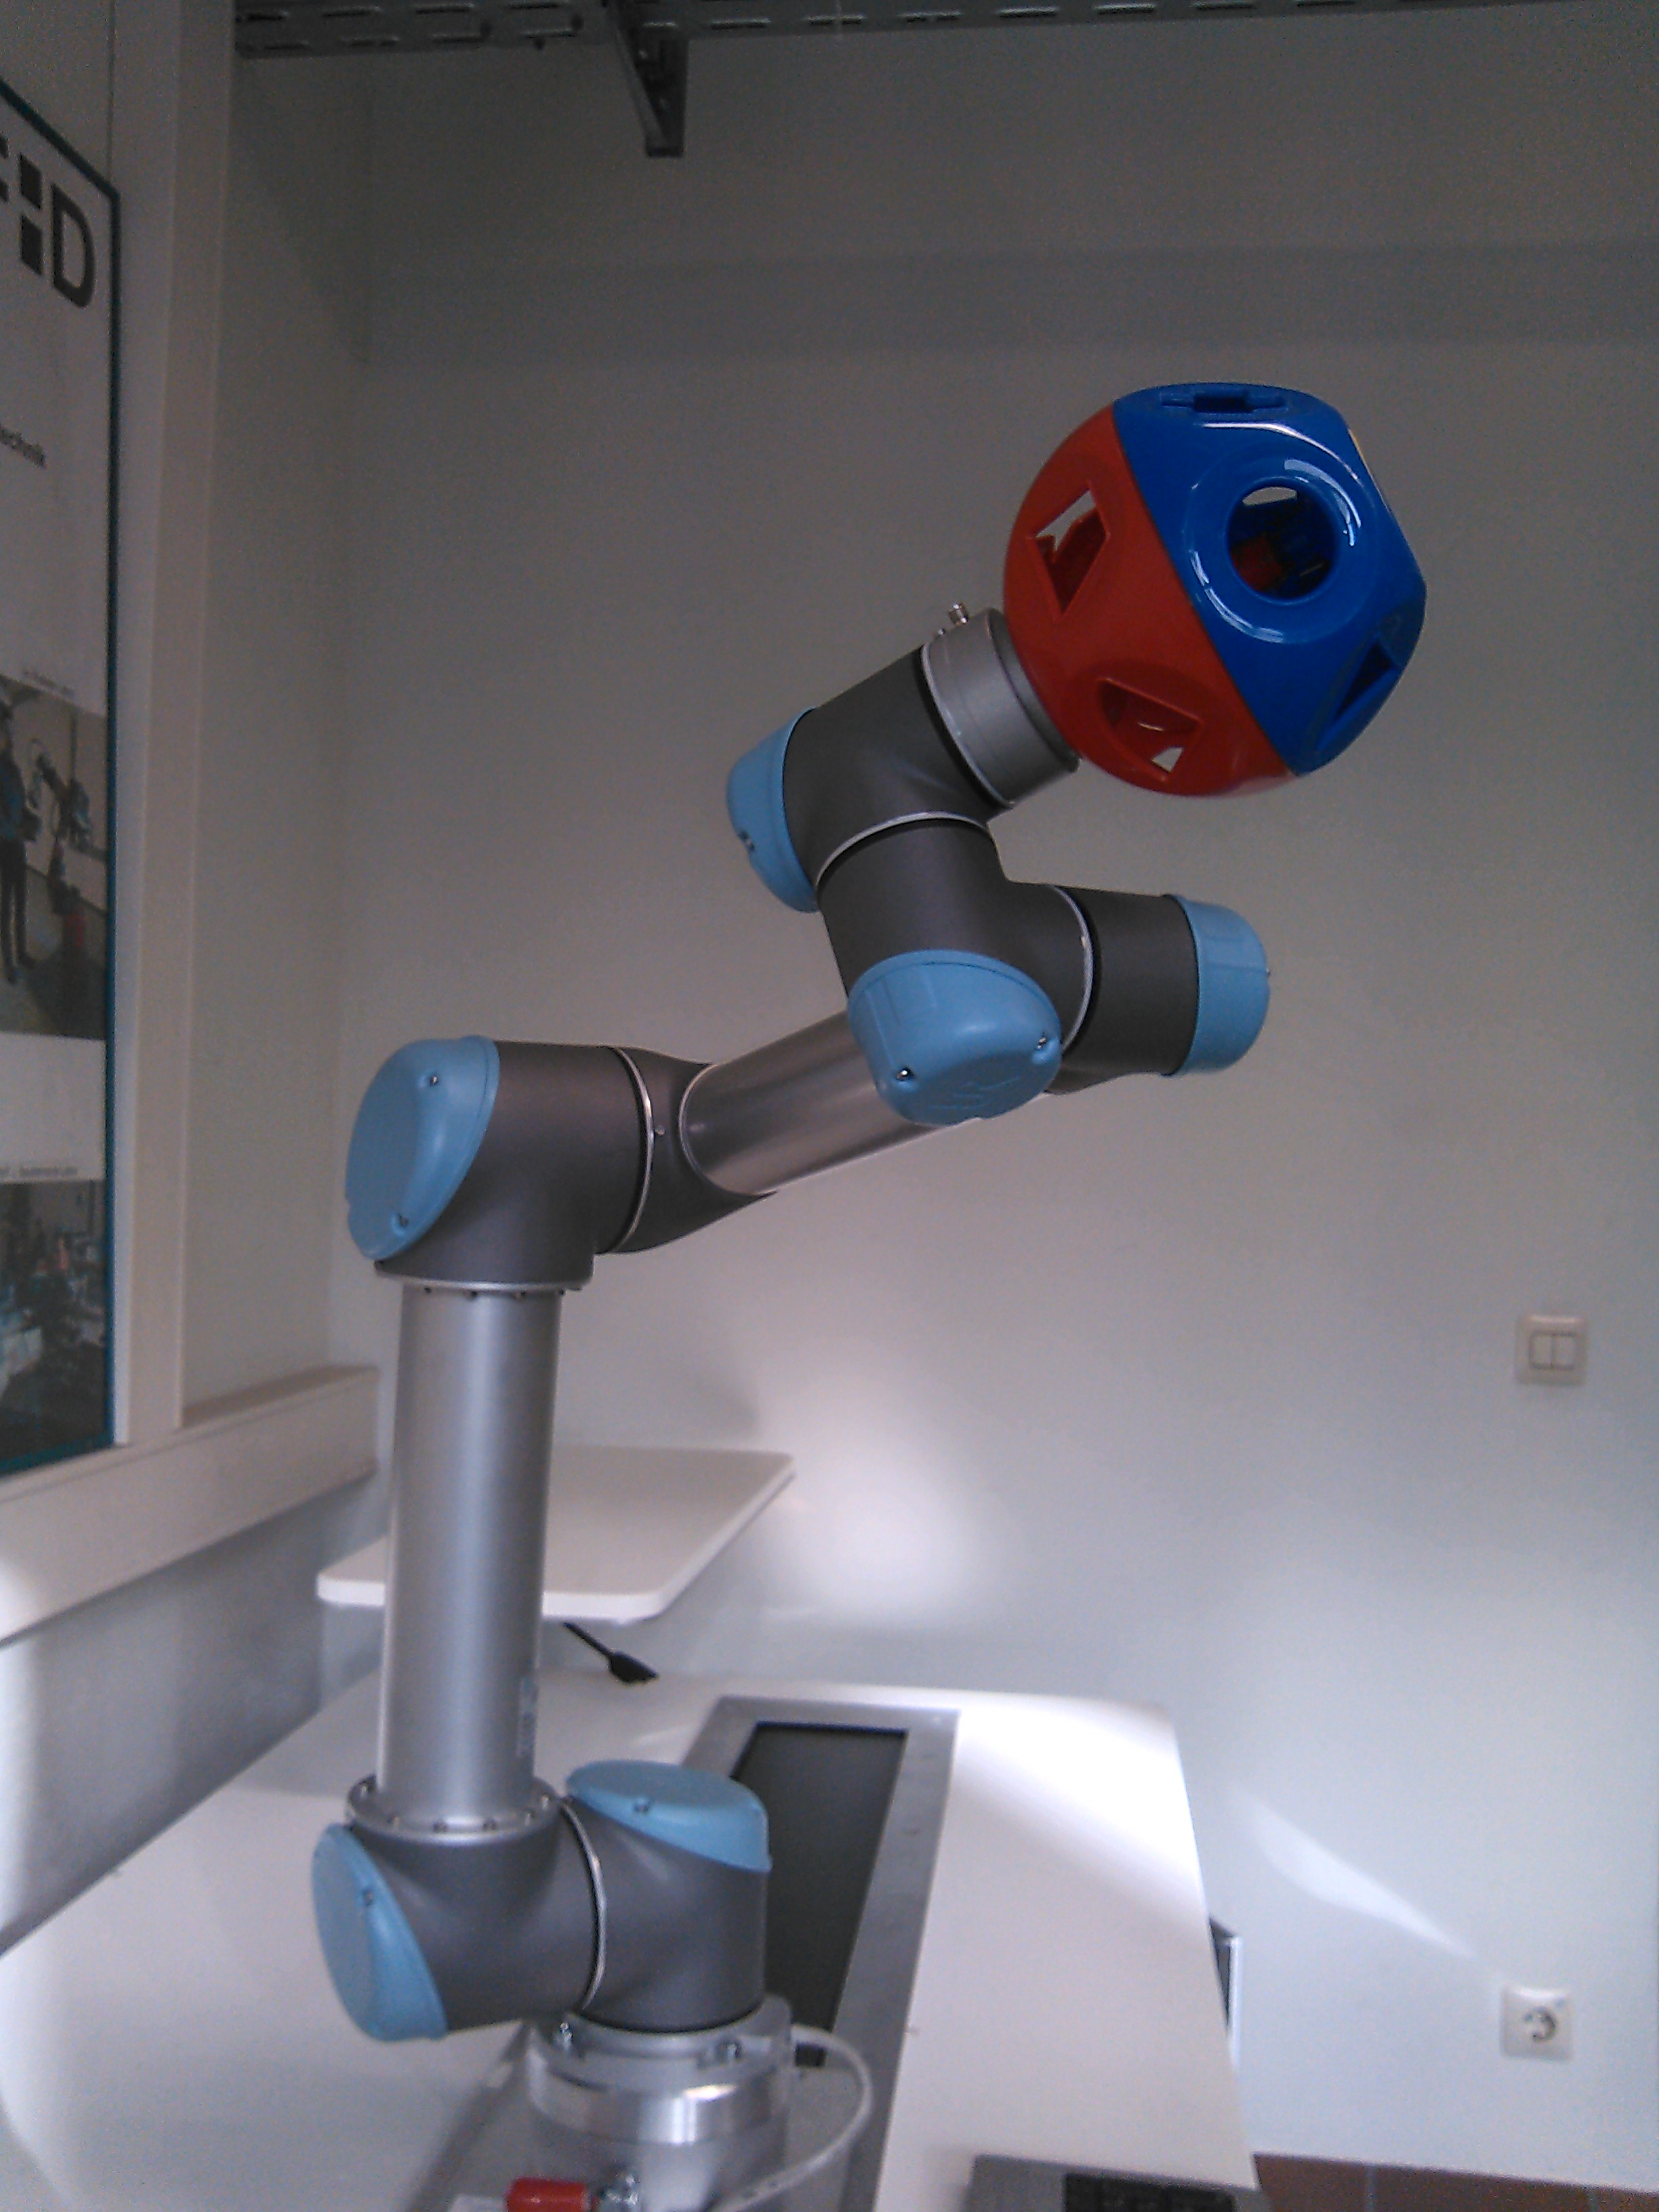
\includegraphics[width=0.4\textwidth]{pic/ur5_robot.jpg}
      \caption[UR5 Roboter]{Abbildung zeigt den UR5 Roboter von Universal Robots}
      \label{fig:schnittstellen_schichten}
\end{figure}

Der Roboter besitzt sechs Gelenke, die ihm einen 360° Arbeitsbereich mit einem Radius von ca. 85 cm ermöglichen. Der Roboterarm hat eine Tragfähigkeit von 5 kg. In den Motoren der einzelnen Gelenke sitzt auch gleichzeitig die Steuerung des Gelenks. Die Hardware des Roboters wird von einem Linux Rechner, der sich in der Nähe befindet, angesprochen.
Die Festplatte für das System ist eine Speicherkarte, die leicht ausgetauscht werden kann.\\
Der Linux Rechner besitzt zehn digitale Eingänge, zehn digitale Ausgänge, vier analoge Eingänge, zwei analoge Ausgänge, die zum Steuern des Roboters benutzt werden können. Des weiteren besitzt der Roboter einen Netzwerk Anschluss, über dem eine Verbindung zu einem oder mehreren Rechnern möglich ist.
\\\\
Um den Rechner anzusprechen, existiert bei Lieferung ein Touch Tablet(siehe Abbildung \ref{fig:tablet_picture}), das für das Linux System den visuellen Output gibt. Es ist möglich, über USB eine Tastatur anzuschließen, um nicht bei Texteingabe das Touch Tablet benutzen zu müssen.
\\
Beim Starten des Systems wird auch automatisch die Software für den Roboter gestartet. Die Software nennt sich Polyscope und wurde in Java geschrieben. Diese Software verbindet sich per \ac{TCP/IP} auf den URController (\ref{sec:ur_control_gru}). Ein Server Programm, dass als Schnittstelle von dem Linux System zu dem Roboter dient.

\subsection{Grundlegendes}
\label{sub:ur_update_gru}

Die Polyscope Software läuft im normalen Modus und dem administrativen Modus. Der normale Modus ermöglicht, es Programme zu erstellen, laufen zu lassen und Grundeinstellungen vorzunehmen. Außerdem kann die Polyscope Software aktualisiert werden.
\\\\
\textbf{System aktualisieren}\\
Zwei Arten von Updates sind hier zu unterscheiden. Zum einen kann das Linux System aktualisiert werden. Dies ist über den Paketmanager des Systems möglich oder wenn man das neueste Image von Universal Robots herunterlädt und das System neu überspielt. Zum Updaten gibt es eine Dokumentation, beiliegend auf der CD.

\section{Programmierschnittstellen vom UR5}
\label{sec:programm_api_uebersicht_gru}

Der UR5 Roboter kann auf drei Ebenen angesprochen werden.\\

\begin{itemize}
\item Polyscope
\item URScript
\item C-API\footnote{\ac{API} ist eine Schnittstelle um eine Software mit einer anderen Software zu verbinden. Die Schnittstelle in Form eines Programmteils wird öffentlich gemacht und dokumentiert. Die externe Software benutzt diesen Programmteil um die Software mit der Schnittstelle zu nutzen.}
\end{itemize}

\begin{figure}[H]
  \centering
    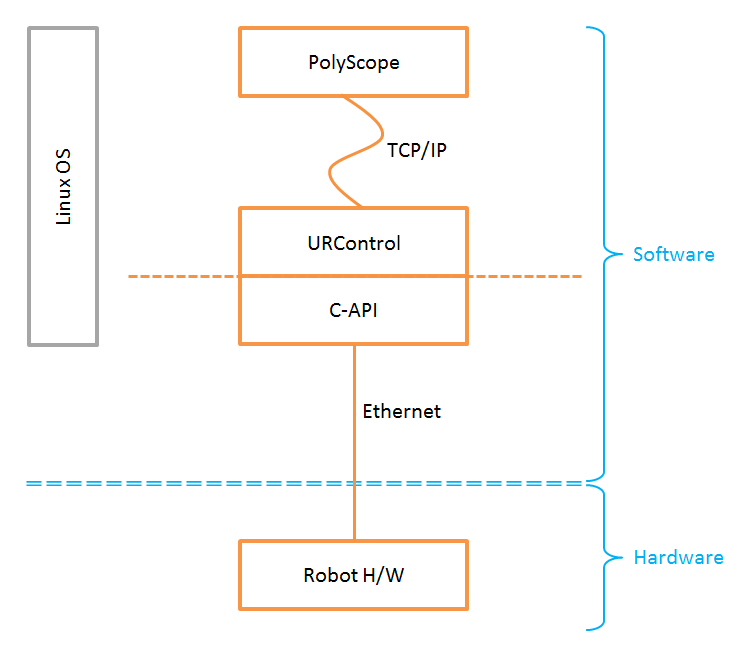
\includegraphics[width=0.8\textwidth]{pic/ur_programming_levels.png}
      \caption[Schichten der Software Schnittstellen]{Übersicht über die
      Schichten der bestehenden Software Schnittstellen des UR5 Roboters}
      \label{fig:schnittstellen_schichten}
\end{figure}

In dieser Arbeit wird versucht, über alle diese Ebenen den Roboter anzusprechen.
Es wird außerdem, aufbauend auf URScript, ein eigener Adapter entwickelt, um eine neue Möglichkeit zu untersuchen, den Roboter anzusteuern. Dieser Adapter wird sich, wie die Polyscope Schnittstelle per \ac{TCP/IP} auf den URController verbinden (siehe Abbildung \ref{fig:schnittstellen_schichten}).
Der Adapter wird für die Programmiersprache Python entwickelt. Gründe hierfür werden im Kapitel für diese Schnittstelle erörtert(siehe \ref{sec:urscript_adapter})

\subsection{Kriterien für die Bewertung der Schnittstellen}
\label{sub:criterias_of_solutions_kon}

Die Schnittstellen werden wie folgt bewertet:

\begin{itemize}
\item Programmierbarkeit
\item Interaktion mit Programm,
\item Möglichkeit zu Debuggen und Testbarkeit
\item Aufwendung
\end{itemize}

Wie schwer ist es, ein Programm für die einzelnen Schnittstellen zu entwickeln?
Kann der Mensch das Programm intuitiv bedienen? Wichtig hierbei ist, dass der Mensch mit dem Roboter kommunizieren kann. Dies geschieht am besten, wenn der Mensch nichts kryptisches eingeben muss. Er braucht anwenderfreundliche Programme.
\\\\
Beim Entwickeln von Programmen ist es wichtig, dass der Entwickler Fehler im Programm entdeckt, um diese schnell zu beheben.
Je größer und komplexer das Programm wird, desto schwieriger wird es, Fehler zu entdecken. 

\section{URController}
\label{sec:ur_control_gru}

Der URController ist eine Server Anwendung, die auf dem Rechner des Roboters läuft. 
Dieser Controller dient als Schnittstelle, zwischen der Roboter Hardware und der Software, die das Roboterprogramm liefert. 

\subsection{Konfiguration des URControllers}
\label{urcontrol_rci_gru}

Den URController kann man konfigurieren. Die Konfigurationsdatei ist abgelegt im folgenden Verzeichniss:
\begin{lstlisting}
\root\.urcontrol\urcontrol.conf
\end{lstlisting}

Beim Starten des Controllers wird diese Konfigurationsdatei eingelesen.
Hier werden wichtige Einstellungen vorgenommen, die zu den jeweiligen Modellen der UR5 oder UR10 Serie gehören. Hier ist ein Ausschnitt der Konfigurationsdatei zu sehen
\\
\begin{lstlisting}[caption={Ausschnitt aus der Datei urcontrol.conf zur Vorkonfigurierung des UR5 Roboters}, label=lst:ur5_conf ,captionpos=b]
[DH]
a = [0.00000, -0.42500, -0.39243,  0.00000,  0.00000,  0.0000]
d = [0.08920,  0.00000,  0.00000,  0.10900,  0.09300,  0.0820]

[Link]
mass = [3.7000, 8.3930, 2.2750, 1.2190, 1.2190, 0.1879]     # Series 3 with tool
gravity = [0, 0, 9.82]          # upright mounting
[Config]
# masterboard_version, 0 = Zero-series, 1 = One-series, 3 = Pause function enabled, 4 = first cb2 version, 5 = ur10 support added
masterboard_version = 4

[Hardware]
controller_box_type = 2 # 1=CB1, 2=CB2UR5, 3=CB2UR10
robot_type = 1  # 1=UR5, 2=UR10
robot_sub_type = 1
\end{lstlisting}

\subsection{Echtzeit-Schnittstelle}
\label{urcontrol_rci_gru}

Die Echtzeit-Schnittstelle ist eine \acs{TCP/IP} Schnittstelle, die im 125Hz Takt Datenpakete an die verbundenen Clients sendet. Diese Schnittstelle kann keine Daten von den Clients empfangen. Wenn man diese Datenpakete auslesen will, muss man die einzelnen Datentypen in dem Paket parsen\footnote{Parser: Informationen zerlegen, entsprechend interpretieren und bereitstellen.}. Eine Besonderheit ist noch, dass die Byte-Reihenfolge der Datenpakete im Big-Endian\footnote{Das Big Engian Format ist die Festlegung der Byte-Reihenfolge, wie das Computersystem Speicherbereiche interpretieren und beschreiben soll. Dieses Format legt fest, dass das höchstwertige Byte an der kleinsten Speicheradresse liegt.} über das Netzwerk übertragen werden. Da der Unix Rechner und der Client Rechner die Byte-Reihenfolge Little-Endian\footnote{Wie bei Big-Endian Format legt das Little-Endian Format die Byte-Reihenfolge fest. Mit Little-Endian jedoch wird das niedrigstwertenste Byte an die kleinste Speicheraddresse gesetzt.} benutzen, muss diese für die einzelnen Datentypen umgewandelt werden. Hierfür wurde in C ein Struct\footnote{Ein Struct ist in C/C++ ein Datentyp, der als Container mehrerer variablen verschiender Datentypen dient} geschrieben und eine Funktion, die das Datenpaket für das Struct in die richtige Byte-Reihenfolge umwandelt.

\begin{lstlisting}[caption={Umwandlung der Byte-Order für Packet über die Echtzeit-Schnittstellen }, label=lst:rci_parse ,captionpos=b]
struct ur5_data_rci * parse_ur5_realtime_ci(struct ur5_realtime_ci *ur5_rci, char *buf){
    // ur5_rci points to the struct that will contain the data of the package
    // buf is the recieved Package from the Real Time Interface
    ur5_rci = (struct ur5_realtime_ci*) buf;

    // the first 4 Byte are the message length of the package. the rest of the packages are 8 Bytes long so we can just iterate over all variables in the package 
    ur5_rci->length = ntohl(ur5_rci->length);
    int i;
    for (i = 0; (i < (sizeof(ur5_rci->data_union.data_packed)/sizeof(double))); i++){
        ur5_rci->data_union.data_packed[i] = htobe64(ur5_rci->data_union.data_packed[i]);
    }
    return &ur5_rci->data_union.data;
}
\end{lstlisting}

Die in der CD beiliegende Dokumentation beinhaltet eine die Beschreibung, wie die Schnittstelle angesprochen wird und wie die Daten benutzt werden, um den Roboter zu analysieren. Im Anhang \ref{bewegungsprofile_anhang} sind Beispiele von Bewegungsprofilen, die von der Echtzeit-Schnittstelle ausgelesen wurden, um zu erfahren wie der URController im Gegensatz zu der Software mit der C-API die Bewegungsprofile berechnet.

\subsection{Secondary und Primary Schnittstelle}
\label{urcontrol_spi_gru}

Die Secondary Schnittstelle ist eine \acs{TCP/IP} Schnittstelle, die in einem 60Hz Takt Nachrichten über den Roboter an verbundene Clients sendet.
Die Nachrichten beinhalten Informationen wie z. B. den Roboter Status oder die Positionen der einzelnen Gelenke.

Zusätzlich kann die Secondary Schnittstelle Befehle von verbundenen Rechnern empfangen.
Diese Befehle können URScript Befehle sein. Ein ganzes Programm in URScript geschrieben oder spezielle zugelassene Befehle, die den Roboter Status verändern.

\begin{figure}[H]
  \centering
    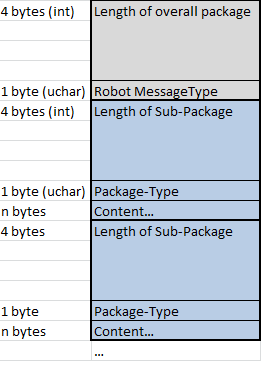
\includegraphics[width=0.5\textwidth]{pic/secondary_datapackage_scheme.png}
      \caption[Schema des Datenpakets gesendet von der Secondary Schnittstelle]{Grobe Darstellung wie die Datenpakete von der Secondary/Primary Schnittstelle gesendet werden.}
      \label{fig:datascheme_of_secondary_interface}
\end{figure}

\subsection{Polyscope}
\label{urcontrol_polyscope_gru}

Polyscope ist eine Anwendung, die auf dem Roboter-Rechner läuft. Die Anwendung verbindet sich per \acs{TCP/IP} auf den URController und sendet URScript Befehle an den Roboter um diesen zu steuern.
Programme die mit Polyscope entwickelt werden, werden im Dateisystem mit der Dateiendung ``.urp'' gespeichert. Weiterer Bezug auf Programme, die mit Polyscope geschrieben werden, werden \ac{URP} bezeichnet.
Diese Anwendung wird auf dem Tablet angezeigt. Hierüber kann man per Toucheingabe ein neues \acs{URP} erstellen. Dieses Programm wird zur Laufzeit in ein Script umgewandelt. Die Polyscope Software schickt nun in Schritten die einzelnen Script-Befehle an den URControl, der diese ausführt. Im Programmbaum kann eingesehen werden, an welchem Schritt sicht das Programm befindet.

\section{C-API}
\label{sec:rest_prinzip_gru}

Die C-API ist von der Firma Universal Robots eine zur Verfügung gestellte C Library\footnote{Library/Modul ist gekapselter Softwarecode, der in anderen Programmen wiederverwendet werden kann.} mit einer Header Datei, die etwaige Funktionen der Library erklärt. Die Header Datei enthält nicht alle Funktionen, somit sind nicht alle zugänglich. Die C-API erlaubt es, einen eigenen Controller für den Roboter zu entwickeln. Es ist nicht möglich, dass mehrere Anwendungen mit der C-API sich gleichzeitig mit dem Roboter verbinden. 
Der URController muss deshalb vor ausführen des eigenen Controllers ausgeschaltet werden. Es schließen sich also die Programmiersprache URScript und ein eigener Controller zunächst aus. Es könnte ein eigener Controller entwickelt werden, der die Befehle in URScript selbst interpretiert und diese wie bei dem URController ausführt. So könnte man die vorhandene Sprache nehmen und diese sogar erweitern.

\subsection{Kontrollstruktur}
\label{capi_control_loop_gru}	

Die C-API ermöglicht es, eine Verbindung zum Roboter zu öffnen und über eigene Funktionen Befehle abzuschicken. Dies erfolgt in einem streng festgelegten Muster.

\begin{lstlisting}[language=C,caption={Beispiel der Kontroll-Struktur}, label=lst:robot_control_loop,captionpos=b]
  while(!endcondition) { // At ROBOT_CONTROLLER_FREQUENCY times per second
    robotinterface_read_robot_state_blocking();
    robotinterface_get_actual_positions(&positions);
     // >>> various calculations <<<
    robotinterface_command_position_velocity_acceleration( xxx, yyy, zzz);
    robotinterface_send_robot_command();
  }
\end{lstlisting}

Die Funktion \sona{robotinterface\_read\_state\_blocking()} startet den Bereich, in dem Datenabfragen an den Roboter gestellt werden können. Daten wie z. B. Temperatur der Motoren, der Stand der Gelenke, die Geschwindigkeit der Gelenke etc. In der Dokumentation beiliegend zu dieser Arbeit sind alle Daten noch einmal aufgelistet. Nachdem die Daten abgefragt wurden, kann mit C-API Funktionen Position, Geschwindigkeit und Beschleunigungswerte übermittelt werden, die der Roboter durch seinen Regler auszuführen versucht.\\
Es können jedoch keine Wegpunkte festgelegt werden, die dann automatisch vom Roboter angefahren werden. Dies muss der Entwickler selbst 
berechnen. 
Es gibt mehrere Verfahren, wie Wegpunkte angefahren werden können (\ref{sub:bewegungsprofile_gru}). In dieser Arbeit sind \ac{PTP}-Verfahren und Linear Verfahren getestet worden.
\\\\
Zum Abschluss wird die Funktion \sona{robotinterface\_send()} aufgerufen, die dafür sorgt, dass der Acht-Millisekundentakt eingehalten wird und die Befehle an den Roboter weitergeleitet werden. Falls die acht Millisekunden überschritten werden, wird der Roboter in einen Sicherheitsmodus gesetzt und angehalten.
\\
Wenn so etwas im URController passiert, kann der Anwender diesen wieder abschalten, sobald alles in Ordnung ist. Dies muss mit der C-API selbst geschrieben werden. Die C-API liefert hierfür auch Funktionen. Damit die richtigen Richtlinien aber auch eingehalten werden, muss von dem Wechsel des Sicherheitsmodus in den normalen Modus eine Benutzerabfrage verlangt werden.

\subsection{Bewegungsprofile}
\label{sub:bewegungsprofile_gru}

In der Robotik gibt es drei wesentliche Verfahren, wie man den Roboter zwischen zwei Punkten bewegen kann. 

\begin{itemize}
\item \ac{PTP}
\item Linear
\item Circular
\end{itemize}

\begin{figure}[H]
  \centering
    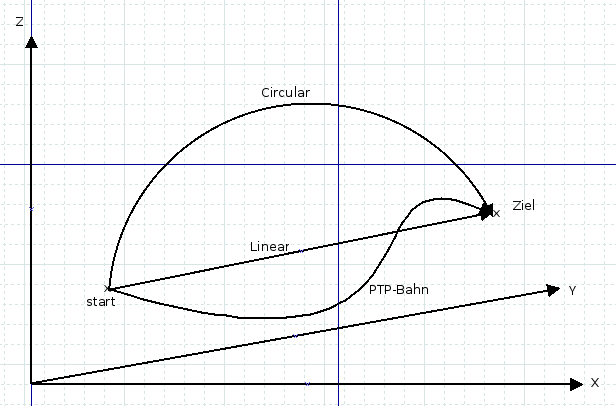
\includegraphics[width=0.8\textwidth]{pic/bewegungsarten.png}
      \caption[Bewegungsarten in Robotik]]{Übersicht über drei verschiedenen Bewegungsarten in der Robotik}
      \label{fig:bewegungsarten}
\end{figure}

Für die C-\ac{API} wurde das \ac{PTP} und das Linear-Verfahren umgesetzt. Die Informationen für die Berechungen sind entnommen aus der Lektüre \sona{Industrieroboter von Wolfgang Weber}\cite{WW-2013}.
\newpage
\textbf{\acs{PTP}-Verfahren}
\\\\
Um den Roboter bestimmte Wegpunkte abfahren zu lassen, muss man die Bewegungsprofile selbst berechnen und ǘber die C-API an den Roboter im 125Hz Takt übergeben. Das \ac{PTP}-Verfahren setzt dabei voraus, dass die einzelnen Positionen der Gelenke bekannt sind. Die Positionen sind die Achs-Werte. Der Wert ist angegeben in Radiant. Auch die Zielposition ist in Achs-Werten anzugeben.
\\\\
\textbf{Linear-Verfahren}
\\\\
Das Linear-Verfahren bedeutet den Roboter von dem \ac{TCP} Punkt aus zu bewegen. Die Bewegung des Roboters wird so berechnet, dass der \ac{TCP} sich linear zum Zielpunkt bewegt(siehe Abbildung \ref{fig:bewegungsarten}).
Um die Berechnung durchzuführen, muss die Position des \ac{TCP} im Raum(kartesische Koordinaten) bekannt sein, um eine Strecke zu einem Zielpunkt abfahren zu können. Der UR5 Roboter kann aber nur Positionen in Achs-Ebene verarbeiten. Deswegen muss zuerst eine Berechnung von Achs-Ebene in kartesische Koordinaten und nach der Berechnung der Strecke wieder zurück auf Achs-Ebene erfolgen.

\section{Eigene Adapter-Schnittstelle aufbauend auf URScript}
\label{sec:urscript_adapter}

Die Secondary Schnittstelle (\ref{urcontrol_spi_gru}) kann benutzt werden, um einzelne Scriptbefehle an den Roboter zu senden. Auf diesem Prinzip aufbauend, kann ein Adapter für jede Programmiersprache entwickelt werden, der die Befehle an den Roboter sendet. Dadurch kann nun ein Anwendungsprogramm in dieser Sprache mit all seinen Vorteilen entwickelt werden.
\\\\
In dieser Arbeit wurde dafür Python gewählt. Gründe hierfür sind:

\begin{itemize}
\item weit verbreitete Programmiersprache
\item ein vorhandener Parser für die Secondary Schnittstelle
\item viele vorhandene Software-Bibliotheken
\item höhere Sprache als z.B C und somit etwas leichter zu programmieren
\end{itemize}

Da, aufbauend auf dieser Arbeit, eventuell mit dem Roboter weitergearbeitet wird, wurde eine Sprache genommen, die weit verbreitet ist. Python ist eine Sprache die nicht so Hardware nah ist, dass man sich um Speicherbelegung kümmern muss, aber den Code schnell ausführt.
Das Open-Source Project ROS\footnote{ROS: Robot Operating System ist ein Open Source Project mit mehreren Software-Bibliotheken um Robotersteuerung zu abstrahieren und das Ansprechen von Robotern zu vereinfachen.} hat für den UR5 eine Schnittstelle entwickelt, bei der schon die Pakete der Secondary Schnittstelle geparsed werden. Das Projekt ist öffentlich, so konnte dieser Code-Abschnitt in die Arbeit übernommen werden.